\newpage
\section{Demonstration}
In this chapter, the prototype is shown demonstratively to highlight the purpose and workings of the code generator. By adjusting the constants in the generator.rs file, it is possible to apply the generator to several similarly constructed databases. The test data in this demonstration is the same database as in the development and testing of the prototype. This is a formatted version of an official Wikipedia dump from September 20th, 2022 \parencite[see][n.p.]{wikimedia_enwiki_nodate}.
\subsection{Database preparations}
The Wikipedia dump is provided in one or more compressed .bz2 files. With the help of an etree of lxml a parser can be built, with which the title and content of each entry can be extracted. Many of the entries are so-called redirects, which are irrelevant for a full-text search and are filtered out (code \ref{code:wiki-csv}, 54). Otherwise, the title and content are written to a CSV file, and further, the longest title and text entries as well as the total amount of entries are being kept track of.
\begin{codeenv}
    \captionof{mycapcode}{Wikipedia as csv}
    \label{code:wiki-csv}
    \lstinputlisting[language=Python, linerange={39-65}]{code/wikidump_sqlserver/convert_wiki_to_csv.py}
    \centerline{Source: convert\_wiki\_to\_csv.py}
\end{codeenv}
When running the script a total of 6,703,714 entries were written in a total runtime of 58 minutes and 14 seconds.\\
Based on the values of the longest title and text a table with a unique id is created. Since the CSV does not contain an id, a temporary view is created into which a bulk insert is executed. The path to the file has been redacted afterward.
\begin{codeenv}
    \captionof{mycapcode}{Insert into SQL server}
    \label{code:wiki-sql}
    \lstinputlisting[language=SQL]{code/wikidump_sqlserver/create_article.sql}
    \lstinputlisting[language=SQL]{code/wikidump_sqlserver/create_view.sql}
    \lstinputlisting[language=SQL]{code/wikidump_sqlserver/bulk_insert.sql}
    \centerline{Source: create\_article, create\_view, bulk\_insert}
\end{codeenv}
Using this \ac{SQL}, all entries were successfully loaded within 41 minutes and 57 seconds. The graphical interface of the Microsoft SQL Server Management Tool then enabled an effortless full-text index creation.
\subsection{Use the prototype}
To use the prototype the \ac{SQL} server must be started and the website including the code generator is started by running the command \lstinline$cargo run$ in the project folder. On localhost:8080 a minimal website with a search field is now visible, where you can enter any request in the custom query language.
\begin{figure}[H]
    \caption{Search field}
    \label{fig:search}
    
\includegraphics[width=0.9\textwidth]{search_field.png}
    \\
    \centerline{Source: Own prototype}
\end{figure}
For example, if you enter the command \lstinline[language=Fulltext-Search]$@near:space, dog, 10:$ you will be redirected to a result page where either the search results or an error message will be displayed. In this case, three matching results are displayed sorted by rank. For each result, the title and rank are displayed and the title can be clicked on to be redirected to the relevant Wikipedia article.
\begin{figure}[H]
    \caption{Results for space dogs}
    \label{fig:space-dog}
    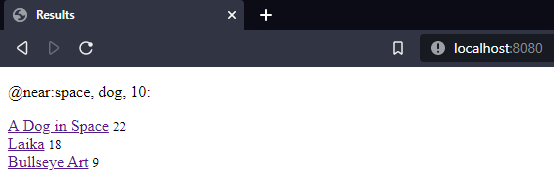
\includegraphics[width=0.9\textwidth]{dog-space-results.png}
    \\
    \centerline{Source: Own prototype}
\end{figure}
The actual generated \ac{SQL} can be looked up in the prototype files if needed. If an incorrect command is entered, the error message thrown in the generator is displayed. For example, the command \lstinline[language=Fulltext-Search]$@weighted:cat, 0.5, dog, 0.8:$ should not be processed as the weights do not add up to exactly 1.
\begin{figure}[H]
    \caption{Weight error}
    \label{fig:weight-error}
    
\includegraphics[width=0.9\textwidth]{weight-error.png}
    \\
    \centerline{Source: Own prototype}
\end{figure}
For demonstration purposes, a complicated search query with multiple functions and nested search terms can also be submitted. A search for apple but without the presence of the terms company or Steve Jobs in combination with a term that has the same meaning as fruit can be formulated in the query language as \lstinline[language=Fulltext-Search]$@contains:apple -(company | "Steve Jobs"): + @thesaurus:fruit:$.
\begin{figure}[H]
    \caption{Results for fruit apples}
    \label{fig:apple-fruit}
    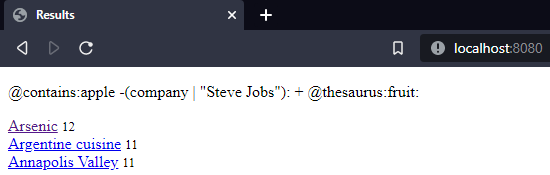
\includegraphics[width=0.9\textwidth]{apple-result.png}
    \\
    \centerline{Source: Own prototype}
\end{figure}
The first result 'Arsenic' describes a chemical element that is listed because of several sentences in the article mentioning its occurrence in apple juice and other fruit juices. Note that it may not be the very best result expected as the test data does not seem to contain every single Wikipedia article, only a large amount.